\documentclass{beamer}

\beamertemplatenavigationsymbolsempty

\usepackage{etex}
% packages required  by CVMono
\usepackage{mathptmx}
\usepackage{helvet}
\usepackage{courier}
\usepackage{type1cm}
\usepackage{makeidx}
\usepackage{graphicx}
\usepackage{multicol}
\usepackage[bottom]{footmisc}
\usepackage{placeins}



%%%
\usepackage[UTF8x]{inputenc}
\usepackage[german,english]{babel}
\usepackage{amsmath}
\usepackage{amssymb}
%\usepackage{amsthm}
\usepackage{pifont}% for checkmarks \ding{51}
\makeatletter
\@ifclassloaded{beamer}{}{\usepackage{paralist}}
\makeatother
\usepackage{float}
\usepackage{adjustbox}

\usepackage[%
    font={small,sf},
    labelfont=bf,
    format=hang,    
    format=plain,
    margin=0pt,
    width=0.8\textwidth,
]{caption}
\usepackage[list=true]{subcaption}
%\usepackage{alltt}

% symbols for the naturals (\mathbbm{N}), integers (\mathbbm{Z}), etc.
\usepackage{bbm}

% nice tables (read the accompanying docs!)
\usepackage{booktabs}
\usepackage{hyperref}% for bookmarks in PDF file
\usepackage{url}%showing url in bibtex
% source code and diagrams
\usepackage{tikz}
\usepackage{tikz-timing}

% code and monostace
\usepackage{listings}
\usepackage{fancyvrb}
\usepackage{fixltx2e}
\usepackage{textcomp}

\usepackage{datetime}



\usepackage{tikz}
\usepackage{import}

% extract lemmas, inserted lemmas
\usepackage{verbatimcopy}
%% "touch foo.ext" before first use
\VerbatimCopy{lem_def_summary}{lem_def_summary_final}

% inference rules
\usepackage{mathpartir}

\let\proof\relax
\let\endproof\relax
\usepackage{amsthm}

% set literals, \Set{ ... | ... }, \Set{ ..., ..., ..., ... }
\usepackage{braket}

% interval literals, \interval{...}{...}, \interval[open left]{...}{...} etc
\usepackage{interval}
\intervalconfig{
	soft  open  fences,
	separator symbol=:,
}

\usepackage{import}
\usepackage{bm}

% \centernot : like \not, but better alignment
\usepackage{centernot}

% has nice things like \cmark and \xmark
\usepackage{pifont}
\usepackage{wasysym}


\usepackage{multirow}
\usepackage{nameref}

% has multiple references grouped together in clever ways; \cref
\usepackage[capitalise]{cleveref}

% manipulates strings
\usepackage{xstring}
%\theoremstyle{definition}
%\newtheorem{definition}{Definition}
%\newtheorem{lemma}{Lemma}
%\newtheorem{theorem}{Theorem}

% note: the next 2 environments are used only in sysbook; have to be adapted wrt to the style reference
\newtheorem{invariant}{Invariant}
\newtheorem{ccond}{Context Condition}

% make float placement on top the default:
\floatplacement{figure}{t}
\floatplacement{table}{t}
\renewcommand{\floatpagefraction}{0.8}

% tikz
\tikzset{timing/slope=0.1}
\tikzset{timing/.style = {y=2.5ex, x = 4.0ex}}

% other
\graphicspath{{figures/}}
\bibliographystyle{alpha}

% remove later
\newcommand{\typo}[1]{\textcolor{blue}{\textbf{#1}}}
\newcommand{\bbox}[1]{\fcolorbox{blue}{white}{#1}}

%%%%%%%%%%%%%%%%%%%%%%%%%%%%%%%%%%%%%%%%%%%%%%%%%%%%%%%%%%%%%%%%
% Define your desired shortcuts here:
\mathchardef\hy="2D
\newcommand{\cm}{\mbox{,}}
\newcommand{\setB}{\mathbb{B}}
\newcommand{\setN}{\mathbb{N}}
\newcommand{\setZ}{\mathbb{Z}}
\newcommand{\setR}{\mathbb{R}}
\newcommand{\setS}{\mathbb{S}}
\newcommand{\B}{\mathbb{B}}
\newcommand{\N}{\mathbb{N}}
\newcommand{\R}{\mathbb{R}}
\newcommand{\nat}{\mathbb{N}}
\newcommand{\Z}{\mathbb{Z}}
\newcommand{\NOT}[1]{\overline{#1}}
\newcommand{\AND}{\land}
\newcommand{\OR}{\lor}
\newcommand{\Sum}{\sum\limits}
\newcommand{\tmod}{\mathrel{\mathrm{tmod}}}
\newcommand{\pskip}{\smallskip\par\noindent}
\newcommand{\ignore}[1]{\relax}
\newcommand{\figscale}{0.834}
%\renewcommand{\pskip}{\smallskip\bbox{\mbox{\quad}}\par\noindent}
\newcommand{\smalltt}[1]{\text{\small\texttt{#1}}}
\newcommand{\super}[1]{\textsuperscript{#1}}
\newcommand{\sub}[1]{\textsubscript{#1}}
\newcommand{\langlett}{{\fontfamily{cmbr}\selectfont\textlangle}}
\newcommand{\ranglett}{{\fontfamily{cmbr}\selectfont\textrangle}}
\renewcommand{\theFancyVerbLine}{\text{\small\arabic{FancyVerbLine}:}}
\renewenvironment{verbatim}[0]{\Verbatim}{\endVerbatim}

% figures
\newcommand{\tfig}[3]{%
\centering%
\adjustbox{scale = \figscale}{\input{figures/#1.pdf_t}}%
\caption{#3}\label{fig:#2}%
}

\newcommand{\tsubfigV}[3]{%
\subcaptionbox{\label{#2} #3}{\import{figures/}{#1.pdf_tex}}%
}

\newcommand{\includefig}[1]{\import{figures/}{#1.pdf_tex}}


\newcommand{\tschemfig}[4]{%
\figure[tp]%
\addtolength{\subfigcapskip}{0.1in}%
\centering%
\subfigure[\label{fig:#1} symbol]{\trimbox{-0.5\textwidth+0.5\width 0pt 0pt}{\raisebox{#3mm}{\adjustbox{scale = \figscale}{\input{figures/#1.pdf_t}}}}}\\%
\subfigure[\label{fig:#1impl} implementation]{\trimbox{-0.5\textwidth+0.5\width 0pt 0pt}{\raisebox{#4mm}{\adjustbox{scale = \figscale}{\input{figures/#1impl.pdf_t}}}}}%
\caption{#2}\label{fig:#1-all}%
\endfigure%
}

%note: command "remark" is already defined in the style file
%\newcommand{\remark}[1]{\marginpar{\framebox{\parbox[t]{16mm}{
  %\tiny\raggedright #1}}}}
%\newcommand{\oldremark}[1]{\relax}

% code
\fvset{
	frame=lines,
	framerule=0.2pt,
	framesep=4pt,
	resetmargins=true,
	xleftmargin=16pt,
	xrightmargin=16pt,
%	numbers=left,
%	numberblanklines=false,
%	numbersep=-16pt,
	tabsize=0,
	fontfamily=courier,
	fontsize=\small,
	commandchars=\\\@\#
}

\lstnewenvironment{code}
    {\lstset{}%
      \csname lst@SetFirstLabel\endcsname}
    {\csname lst@SaveFirstLabel\endcsname}
    \lstset{
      language=Haskell,
      mathescape = true,
      commentstyle= \sffamily\itshape,
      basicstyle=\small\ttfamily,
      keywordstyle=\color{DarkBlue}\bfseries,
      flexiblecolumns=false,
      basewidth={0.5em,0.45em},
      morecomment=[l]{//},
      numbers = left,
      numberstyle = \color{Gray}\tiny\ttfamily,
      breaklines = true,
      literate={+}{{$+$}}1 {*}{{$*$}}1 {=}{{$=$}}1 {!=}{{$\neq$}}2
               {>}{{$>$}}1 {<}{{$<$}}1 {\\}{{$\lambda$}}1
               {->}{{$\rightarrow$}}2 {>=}{{$\geq$}}2 {<-}{{$\leftarrow$}}2
               {<=}{{$\leq$}}2 {=>}{{$\Rightarrow$}}2
               {>>}{{$\gg$}}1
               {<<}{{$\ll$}}1
               {|}{{$\mid$}}1
               {||}{{$\vee$}}2 {&&}{{$\wedge$}}2
               {@}{{$\circ$}}1
               {?}{{{\color{DarkBlue}{?}}}}1
               {...}{{$\ldots$}}3
    }

% forbids footnotes to travel
%\interfootnotelinepenalty=1000000000
\interfootnotelinepenalty=10000

% theorems of amsthm

% config of the tikz package
\usetikzlibrary{automata,positioning}

%new shorthands

% Tombstone at end of proof (amsthm does this now)
%\renewcommand\endproof{~\hfill\qed}

% std mathcal font
\DeclareMathAlphabet{\mathcal}{OMS}{cmsy}{m}{n}

% new utils
\newcommand{\tikscale}{1.0}

\newcommand{\tbl}[3]{%
\caption{#3}%
\label{tab:#2}%
\centering%
\input{tables/#1}%
}

\newcommand{\tpic}[3]{%
\centering%
\adjustbox{scale = \tikscale}{%
\tikzpicture[%
	>=stealth,%
	shorten >=0.5pt,%
	node distance=2.5cm,%
	on grid,%
	auto,%
	every node/.append style={very thin},%
	every path/.append style={very thin}%
]%
\input{drawings/#1}%
\endtikzpicture}%
\caption{#3}\label{fig:#2}%
}

\newcommand{\tfigscaled}[4]{%
\centering%
\adjustbox{scale = #4}{\input{figures/#1.pdf_t}}%
\caption{#3}\label{fig:#2}%
}

%%% REDUCTION PROOFS
%% units making steps
\newcommand{\MMU}{\mathrm{MMU}}
\newcommand{\SB}{\mathrm{SB}}
\newcommand{\APIC}{\mathrm{APIC}}
\newcommand{\IOAPIC}{\mathrm{IOAPIC}}
\newcommand{\DEV}{\mathrm{DEV}}

%% classes of schedules
\newcommand{\LSBS}{\mathrm{LSBS}}
\newcommand{\ABS}{\mathrm{ABS}}
\newcommand{\REDUCIBLE}{\mathrm{RED}}
\newcommand{\IND}{\mathrm{ORD}}

\newcommand{\IBLOCK}{\mathrm{IBLOCK}}
\newcommand{\CBLOCK}{\mathrm{CBLOCK}}
\newcommand{\EIBLOCK}{\mathrm{EIBLOCK}}
%% 
\newcommand{\sbcomp}[1]{{\overline{#1}}}


%% Makes it into a single word...
\newcommand{\inputsafe}{in\hy safe}
%% communication relations
\DeclareMathOperator{\fwdsync}\vartriangleright
\DeclareMathOperator{\rsync}{{\ooalign{$\vartriangleright$\cr\kern0.04em
  $\ast$\cr}}}
\DeclareMathOperator{\sync}{\blacktriangleright}
\DeclareMathOperator{\talks}{\sync\!\!\!\!\!\fwdsync}
\DeclareMathOperator{\rtalks}{\sync\!\!\!\!\!\rsync}
\DeclareMathOperator{\backsync}{\vartriangleleft}
\DeclareMathOperator{\leaksync}{\blacktriangleright_2}

%% memory update 
\DeclareMathOperator*{\updatedby}{\circledast}
\DeclareMathOperator*{\uninfupdatedby}{\circledcirc}


%% function restriction
\newcommand\restr[2]{{% we make the whole thing an ordinary symbol
  \left.\kern-\nulldelimiterspace % automatically resize the bar with \right
  #1 % the function
  \vphantom{\big|} % pretend it's a little taller at normal size
  \right|_{#2} % this is the delimiter
  }}
%% intersects
\DeclareMathOperator*{\intersects}{\dot\cap}
%% List comprehension, taken from braket
{\catcode`\|=\active
  \xdef\List{\protect\expandafter\noexpand\csname List \endcsname}
  \expandafter\gdef\csname List \endcsname#1{\left[%
     \ifx\SavedDoubleVert\relax \let\SavedDoubleVert\|\fi
     \:{\let\|\SetDoubleVert
     \mathcode`\|32768\let|\SetVert
     #1}\:\right]}
}

%% absolute/length
\providecommand{\abs}[1]{\lvert#1\rvert}
\providecommand{\len}[1]{\lvert#1\rvert}

%% from
\newcommand{\from}\leftarrow


%% Aliases for readablity
\newcommand{\Iota}I

%% checkmark and x
\newcommand{\cmark}{\ding{51}}%
\newcommand{\xmark}{\ding{55}}%

%% When the machines agree
\providecommand{\MI}{\ast}
\providecommand{\M}[1]{\MI} %can be replaced by #1 in case we decide to distinguish the machine types after all



%normal red is too bright
\definecolor{red}{HTML}{800000} 

\usetikzlibrary{matrix,shapes,arrows,fit,tikzmark}
%\usepackage{bm}


% \C is used inside figures created by inkscape, which sadly does not have good alignment support for tex.
\newcommand\C[1]{\raisebox{-0.5\height}{\texttt{#1}}} 

\title{My Research}
\author{Jonas Oberhauser}
\date{\today} % Date, can be changed to a custom date
\begin{document}
\begin{frame}
\titlepage % Print the title page as the first slide
\end{frame}

\begin{frame}
\frametitle{Verisoft XT Model Stack}
\begin{center}
 \includefig{modelstack_lowdetail}
 \end{center}
\end{frame}

\begin{frame}
\frametitle{Correctness Proof}
\begin{itemize}
	\item Each layer is implemented in the layer below
	\item Prove between layers:
	\begin{center}
		every execution of implementation at level $i$ in layer $i$ reaches a state 
		``consistent with'' some execution at layer $i+1$
	\end{center}
	\item E.g.: 
	\begin{itemize}
		\item gate level design implements ISA for all programs
		\item compiler implements C+assembler+OS for all programs
		\item \ldots
	\end{itemize}
\end{itemize}
\end{frame}

\begin{frame}
\frametitle{For Single Core: Sysbook}
\scalebox{0.5}{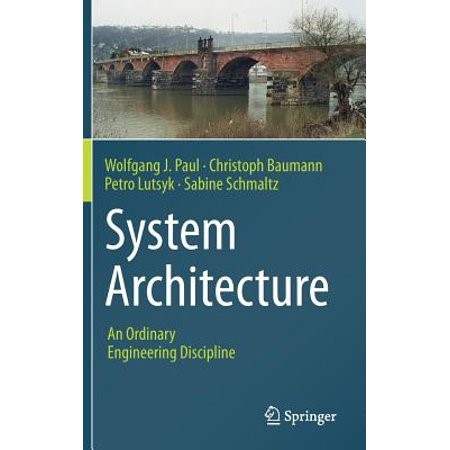
\includegraphics{figures/sysbook}} 
\begin{itemize}
	\item<2-> I only worked on very basic OS kernel
\end{itemize}
\end{frame}


\begin{frame}
\frametitle{My Work: For Multi Core}
\begin{center}
	\includefig{modelstack_mywork}
\end{center}
\end{frame}


\begin{frame}
\begin{itemize}
	\item Main Focus of Talk:
	My Recent Research
	\item \textbf{$=$ Order Reduction}
	\item \textbf{$\ne$ partial} order reduction
\end{itemize}
\end{frame}


\begin{frame}
\frametitle{Naive Concurrent Proof}
\begin{center}
	\texttt{
		\begin{tabular}{l||l}
			t1 = i; & t2 = i; \\
			 i = t1 + 1; &  i = t2 + 1;  \\
		\end{tabular}
	}
\end{center}

\begin{enumerate}
	\item<2-> left side $\equiv \texttt{i++}$
	\item<3-> right side $\equiv \texttt{i++}$
	\item<4-> thus: total effect $\equiv 2\times \texttt{i++}$
\end{enumerate}
\end{frame}

\begin{frame}
\frametitle{Naive Concurrent Proof: Visually}

\begin{center}
		\begin{tabular}{cccc}
			\scalebox{.45}{\includefig{increment_schedule1122}} &  \hspace{0.2em} & \onslide<2->{ \scalebox{.45}{\includefig{increment_schedule1212}}} &  \scalebox{.45}{\onslide<2->{\includefig{increment_schedule1221}}}\\
			\scalebox{.45}{\includefig{increment_schedule2211}} & \hspace{0.2em} & \onslide<2->{\scalebox{.45}{\includefig{increment_schedule2121}}} & \onslide<2->{\scalebox{.45}{\includefig{increment_schedule2112}}}	\\
			& & & \\
			proof works here!   &  &  &  \onslide<2->{\textbf{what about these!?}}	\\
	\end{tabular}
\end{center}

\end{frame}

\begin{frame}
\frametitle{Standard Invariant Based Proofs}
\vfill
General idea:
Whenever some thread $i$ takes the system from state $s$ to $s'$, show that invariant $I$ is maintained
\[ s \overset{i}\longrightarrow s' \  \land \ I(s) \quad \to \quad I(s') \]

\begin{itemize}
	\item Owicky-Gries, CSL, rely-guarantee...
\end{itemize}
\vfill
\onslide<2->{
\begin{center} \scalebox{.55}{\includefig{proof_invariant}} \end{center}}
\vfill

\end{frame}



\begin{frame}
\frametitle{Reduction (Lipton 1975)}
\vfill
Break each thread down into transactions...
\vfill
\begin{center}
	\begin{tabular}{ccc}
		\scalebox{.45}{\includefig{proof_lipton}} &  \hspace{0.2em} & \onslide<2->{ \scalebox{.25}{\includefig{proof_lipton_move}}} \\
		& & \\
		prove correctness only here   &  &  \onslide<2->{prove only commutativity}	\\
	\end{tabular}
\end{center}
\vfill
\end{frame}


%\begin{frame}
%\frametitle{``Formally''}
%\begin{enumerate}
%\item Prove for transaction of a thread $i$
%\[ s_0 \overset{i}\longrightarrow s_1  \overset{i}\longrightarrow \ldots  \overset{i}\longrightarrow s_{n-1} \overset{i}\longrightarrow s_n \  \land \ I(s_0) \quad \to \quad I(s_n) \]
%where $s_0$ is a transaction boundary and none of $s_1$, \ldots, $s_{n-1}$ are
%
%
%\item
%Prove for arbitrary executions: 
%\[ \leftarrow\!(s,i) \ \land \ j \not= i \ \land \ s \overset{i \circ j}\longrightarrow s'  \quad \to \quad s \overset{j \circ i}\longrightarrow s' \]
%and
%\[ \rightarrow\!(s,i) \ \land \ j \not= i \ \land \ s \overset{j \circ i}\longrightarrow s'  \quad \to \quad s \overset{i \circ j}\longrightarrow s' \]
%\end{enumerate} 
%\end{frame}


\begin{frame}
\frametitle{You won't believe what happens next}
\vfill
\begin{center} \scalebox{.55}{\only<1>{\includefig{understanding_vs_disbelief}}\only<2>{\includefig{understanding_vs_disbelief_boss}}\only<3>{\includefig{understanding_vs_disbelief_boss_and_me}}} \end{center}
\vfill
\end{frame}



\begin{frame}
\frametitle{Order Reduction (Ernie Cohen 2006)}
\begin{center}
	\begin{tabular}{ccc}
		\scalebox{.45}{\includefig{proof_lipton}} &  \hspace{0.2em} & \scalebox{.25}{\includefig{proof_lipton_move}} \\
		& & \\
		prove correctness   &  &  \textbf{prove nothing here (!?)}	\\
		and commutativity & & \\
	\end{tabular}
\end{center}
\end{frame}


\begin{frame}
\frametitle{Commutativity By Ownership (2006)}
Dynamic object ownership model: owned by thread $i$ in state $s$
\[ \textit{ownedVars}_i(s) \]
\vfill
\begin{center} \scalebox{.65}{\includefig{proof_cohen}} \end{center}
\vfill
\begin{itemize}
	\item Only shared step can touch shared state
	\item Only shared step can change ownership
	\item Shared step must be first
\end{itemize}
\end{frame}



\begin{frame}
\frametitle{Non-Standard Invariant Proof (VCC)}
\vfill
\begin{center} \scalebox{.65}{\includefig{proof_invariant_coarse}} \end{center}
\vfill
\end{frame}

\begin{frame}
\frametitle{Non-Standard Invariant Proof (VCC)}
Prove for transaction of a thread $i$
\[ s_0 \overset{i}\longrightarrow s_1  \overset{i}\longrightarrow \ldots  \overset{i}\longrightarrow s_{n-1} \overset{i}\longrightarrow s_n  \]
where $s_0$ is a transaction boundary, none of $s_1$, \ldots, $s_{n-1}$ are, and invariants hold
\[ \textit{TB}(s_0)  \ \land \ (\forall k \in [1:n-1]. \ \neg \textit{TB}(s_k)) \ \land \ I(s_0) \]
\begin{enumerate}
\item Invariant is maintained:
\[ I(s_k) \]

\item Also prove commutativity through ownership protocol
\begin{itemize}
	\item After first step $k > 0$:
	\begin{itemize}
		\item \(\textit{accessedVars}(s_k,i) \subseteq \textit{ownedVars}_i(s_k)\)
		\item \(\textit{ownedVars}_i(s_k) = \textit{ownedVars}_i(s_{k+1})\)
	\end{itemize}
	\item even in first step for $j\not=i$:
	\[ (\textit{accessedVars}(s_0,i) \cup \textit{ownedVars}_i(s_1)) \cap \textit{ownedVars}_j(s_0) = \emptyset \]
\end{itemize}
\end{enumerate} 
\end{frame}

\begin{frame}
\frametitle{Baumann (2014)}
\vfill
\begin{center} \scalebox{.65}{\includefig{proof_baumann}} \end{center}
\vfill
\begin{itemize}
	\item + include improved ownership model of Cohen-Schirmer except dynamic read-only
\end{itemize}
\end{frame}

\begin{frame} 
\frametitle{Problem: Locks}
\begin{center}
	\texttt{
		\begin{tabular}{l||l}
			L.lock(); & L.lock();
			\\
			t1 = i; & t2 = i;
			\\	
			i = t1+1; & i = t2+1;
			\\
			L.unlock(); & L.unlock();
		\end{tabular}
	}
\end{center}
\begin{itemize}
	\item each \texttt{L.lock} and \texttt{L.unlock} touches shared state!
	\item two transactions per thread?
	\item<2-> Cohen: formally proves for a particular implementation of monitors as part of order reduction theorem:
	\begin{center}
		``\lstinline[mathescape]{.release()} can be treated like local''
	\end{center}
	\item<3-> What about all other implementations of monitors? What about \lstinline[mathescape]{.acquire()}? What about locks, signals, ... ?
\end{itemize}
\end{frame}



\begin{frame}
\frametitle{Oberhauser (2017)}
\begin{center} \scalebox{.65}{\includefig{proof_oberhauser}} \end{center}
\begin{itemize}
	\item Acquire: only acquire ownership, and
	\[ \textit{accessedVars}(s_k,i) \subseteq \textit{ownedVars}_i(s_{k+1}) \]
	\item Release: only release ownership, and
	\[ \textit{accessedVars}(s_k,i) \subseteq \textit{ownedVars}_i(s_{k}) \]
\end{itemize}
\end{frame}


\begin{frame} 
\frametitle{No Problem: Locks}
\begin{center}
	\texttt{
		\begin{tabular}{l||l}
			L.lock(); \_acq(L,i); & L.lock(); \_acq(L,i);
			\\
			t1 = i; & t2 = i;
			\\	
			i = t1+1; & i = t2+1;
			\\
			L.unlock(); \_rel(L,i); & L.unlock(); \_rel(L,i);
		\end{tabular}
	}
\end{center}
Proof now: 
\begin{itemize}
	\item left side $\equiv \texttt{i++}$ and obeys ownership
	\item right side $\equiv \texttt{i++}$ and obeys ownership
	\item total effect $\equiv 2\times \texttt{i++}$
\end{itemize}
\end{frame}

\begin{frame}
\frametitle{KTH Hypervisor + NIC}
NIC and HV/guest concurrently access queue:
\begin{center} \scalebox{.65}{\includefig{HV_NIC}} \end{center}
\end{frame}

\begin{frame}
\frametitle{Guest vs NIC Race Condition:}
Guest inserts packet while NIC is processing last element:
\begin{center} \scalebox{.45}{\includefig{Guest_vs_NIC_before}} \end{center}
Two possibilities:
\begin{center}
	\begin{tabular}{ccc}
		\scalebox{.45}{\includefig{Guest_vs_NIC_beforeNIC}} &  \hspace{1em} & \scalebox{.45}{\includefig{Guest_vs_NIC_afterNIC}} \\
	\end{tabular}
\end{center}
\end{frame}


\begin{frame}
\frametitle{HV: Clean Up}
HV collects all packets, and restarts NIC if it turned off too early
\begin{center}
\texttt{
	\begin{tabular}{l}
		p = HeadP; // read-read race
		\\
		while (p \&\& p->done) \{ \_acq(*p); // racy read
		\\
		\quad cleanUp(p);
		\\
		\quad if (p->EOQ \&\& p->next) \{
		\\
		\quad \quad p->EOQ = 0;
		\\
		\quad \quad HeadP = p->next; // racy store
		\\ 
		\quad\quad break;
		\\
		\quad \}
		\\
		\quad p = p->next;
		\\
		\}
	\end{tabular}
}
\end{center}
\begin{itemize}
	\item<2-> Entire code is a single transaction and can be verified sequentially!
\end{itemize}
\end{frame}

\begin{frame}
\frametitle{...but does it really work?}
\begin{itemize}
	\item mechanized my version of order reduction in Coq (first mechanized proof of order reduction!)
	\item implemented a small statically typed pointer language in Coq
	\item implemented the code in that language in Coq
	\item verified in Coq that it maintains invariants + satisfies all conditions of theorem	
\end{itemize}
\end{frame}


\begin{frame}
\frametitle{What about speculation?}
\begin{center}
	\texttt{
		\begin{tabular}{l||l}
			do \{ 
			&
			while (1) \{
			\\
			\quad r0,r1 = x,ctx;
			&
			\quad x,ctx = rand(),ctx+1;
			\\
			\quad r2 = y;
			&
			\quad y = rand();
			\\
			\} until (r1==ctx);
		\end{tabular}
	}
\end{center}
\begin{itemize}
	\item speculates that \lstinline[mathescape]{ctx} is unchanged
	\item rolls back otherwise
\end{itemize}
\end{frame}


\begin{frame}
\frametitle{Other Class of Speculation:}
\begin{center}
	\texttt{
		\begin{tabular}{l}
			while (!lock.tryLock()); // data race!
			\\
			t1 = i;
			\\
			i = t1+1;
			\\
			lock.release();
		\end{tabular}
	}
\end{center}
\begin{itemize}
	\item speculates that \lstinline[mathescape]{tryLock} returns 1
	\item rolls back otherwise
\end{itemize}
\end{frame}

\begin{frame}
\frametitle{Oberhauser (2018)}
\begin{center}
	\begin{tabular}{ccc}
		\scalebox{.45}{\includefig{proof_lipton}} &  \hspace{1em} & \scalebox{.25}{\includefig{proof_lipton_move}} \\
		& & \\
		correctness   &  &  \textbf{prove rollbacks succeed}	\\
		and extended ownership & &\\
	\end{tabular}
\end{center}
\begin{itemize}
	\item Left side includes only correct speculation! (\lstinline[mathescape]{tryLock()} always succeeds, \lstinline[mathescape]{ctx} obviously unchanged)
\end{itemize}
\end{frame}

\begin{frame}
\frametitle{Oberhauser (2018)}
\begin{itemize}
\item Extend ownership with ``memory'' of \lstinline[mathescape]{ctx}
\item allowed to read values in memory as if they were owned
\item<2-> Also mechanized in Coq, including the two examples and seqlocks 
\item<2-> Used theorem to conclude in Coq for these examples: ``invariant holds in all reachable states''
\item<3-> Not my day job!
\end{itemize}
\end{frame}

\begin{frame}
\frametitle{But what about preemptive kernel?}
\begin{itemize}
	\item interrupted kernel thread and handler share \emph{registers} 
	\item handler needs to access those registers during process save
	\item obviously no commutativity!
\end{itemize}
\end{frame}

\begin{frame} 
\frametitle{Problem}
\begin{itemize}
	\item In preemptive scheduler, interrupts occur at any point
	\begin{center} 
		\includefig{BlockSuspension}	
	\end{center} 
	\item In cooperative scheduler, interrupts only occur at TB
	\begin{center} 
		\includefig{BlockSuspensionComplete}	
	\end{center} 
	\item<2-> Stored contexts contain data that depends on precise moment of interrupt!
\end{itemize}
\end{frame}

\begin{frame}
\frametitle{Two Solutions (2016)}
\begin{itemize}
	\item $>$6-year PhD of Pentchev
	\item contract runs out late 2014
	\item takes a job in industry
	\item ``will finish my PhD there!''
	\item<2-> takes all his research with him
	\item<3-> Boss (2015): ``he's too busy making money. \textbf{you solve it}''
	\item<4-> early 2016: I have the results
	\item<5-> also early 2016: Pentchev submits dissertation (!)
\end{itemize}
\end{frame}

\begin{frame}
\frametitle{Pentchev vs Oberhauser (2016)}
\begin{tabular}{r|cc}
	& Pentchev & Oberhauser
	\\
\hline Stack P. & local (+) & shared (-)
	\\
IH & one implementation (-) & generic conditions (+)
	\\
ownership & Baumann (-) & dynamic read-only (+)
\end{tabular}
\vfill 
Note: 2016$<$2017, everything uses only shared/local steps
\end{frame}

\begin{frame}
\frametitle{Oberhauser (2016)}
Obvious conditions:
\begin{enumerate} 
	\item don't depend on context
	\item restore state after eret
\end{enumerate} 
\vfill
Not so obvious:
\begin{enumerate}
	\item how to formalize this so it is sound to check only cooperative schedules?
	\item how to deal with parts of state that can not be restored (exception pc)?
\end{enumerate}
\end{frame}

%%Taken from https://tex.stackexchange.com/questions/240542/adding-a-rectangular-box-with-tikz-to-table-beamer

	% Some options common to all the nodes and paths
	\tikzset{   
		every picture/.style={remember picture,baseline},
		every node/.style={anchor=base,align=center,outer sep=1.5pt},
		every path/.style={thick},
	}
	
	\newcommand\marktopleft[1]{%
		\tikz[overlay,remember picture] 
		\node (marker-#1-a) at (.4em,.1em) {};%
	}
	\newcommand\markbottomright[2]{%
		\tikz[overlay,remember picture] 
		\node (marker-#1-b) at (-.4em, .5em) {};%
		\tikz[overlay,remember picture,inner sep=3pt]
		\node[draw=#2,rounded corners,fit=(marker-#1-a.north west) (marker-#1-b.south east)] {};%
	}

%%end Taken




\begin{frame}
Partition into four classes of registers:

\alt<2->
{\alt<3->
	{\begin{center} 
			\includefig{MLayoutPRNonPre}
	\end{center}}
	{\begin{center} 
			\includefig{MLayoutPRPre}
\end{center}}}
{\begin{center} 
		\includefig{MLayoutPR}
\end{center}}
\end{frame} 

\begin{frame} 
Keep track of context with ``dirtiness'' formalism:

\[ d(a) = \begin{cases} \bot & \text{not dirty} \\
\square & \text{contains trash} \\
(r,X) & \text{contains value of register $r$ of thread $X$}
\end{cases} \]

So to restore context of thread $X$:
\begin{align*}
eret \ &\land \ d(epc) = (pc,X) \ 
\\ &\land \ d(emode) = (mode,X) 
\\
&\land \ d(\texttt{t1}) = (\texttt{t1},X)
\\ &\land \ \ldots
\end{align*}
\end{frame} 



\begin{frame} 
Dirtiness Condition 1: \textbf{don't compute with dirty data}

Assume
\[ d(\texttt{t1}) = (r,X) \]

Allowed:
\begin{center}\texttt{y = t1;}\end{center} 

Forbidden:
\begin{center}\texttt{y = t1+t2;}\end{center} 
\end{frame}

\begin{frame} 
Dirtiness Condition 2: \textbf{don't use dirty data}

Assume \[ d(\texttt{t1}) = (r,X) \ \lor \ d(\texttt{t1}) = \square \]

Forbidden:
\begin{center}\texttt{*(t1) = 1;}\end{center} 

Forbidden:
\begin{center}\texttt{if (t1) \ldots}\end{center} 

Forbidden:
\begin{center}\texttt{PTE = t1;}\end{center} 
\end{frame}

\begin{frame} 
Dirtiness Condition 3: \textbf{don't rely on the value of dirty addresses}

Assume 
\begin{align*} d(\texttt{t1}) &= (pc,X) 
\\
\texttt{t1} &= 3
\end{align*}
Allowed:
\begin{center}\texttt{epc = t1, eret;}\end{center} 

Forbidden:
\begin{center}\texttt{epc = 3, eret;}\end{center} 
\end{frame} 

\begin{frame} 
\begin{center}\texttt{
\begin{tabular}{ll||l}
& T & IH \\
\color{gray} 1 &
\{enable interrupts\},	& t1 = epc, \\
\color{gray} 2 &
t2 = t2+1; 	& epc = 3, \\
\color{gray} 3 &
\{disable interrupts\}; & eret;
\end{tabular}
}\end{center}

Works in cooperative scheduler because 
\[ \texttt{epc} = 3 \]
on all interrupts, but in preemptive scheduler
\[ \texttt{epc} = 2 \]
\end{frame}

\begin{frame} 
\textbf{Dirtiness \& invariants}

Invariants must ignore the value of dirty addresses

Allowed:
\[ d(\texttt{t1}) = \bot  \  \land \ \texttt{t1} = 3  \]

Forbidden:
\[ d(\texttt{t1}) = \square \ \land \ \texttt{t1} = 3 \]
\end{frame}


\begin{frame}
\frametitle{Other Work: Weak Memory Reduction (x86-TSO)}
\begin{itemize}
	\item Take any program which obeys the ownership policy
	\item Put a memory barrier between racy store and racy load
	\item $\to$ program has no new behaviors on x86 weak memory model
	\item this is more efficient than current compilers!
	\item Original theorem: Cohen and Schirmer (2010) for simplified processor
	\item<2-> I added operating system support: 
	\begin{itemize} 
		\item inter processor interrupts, 
		\item users that violate ownership policy \& flushing 
		\item misaligned \& differently sized accesses
		\item MMUs if they do not race with OS (this sub-point was solved concurrently in 4-year PhD of Chen)
	\end{itemize} 
	\item<3-> 494 pages....
\end{itemize}
\end{frame}


\begin{frame}
\frametitle{Weak Memory Reduction --- Future?}
\begin{itemize}
	\item Improved ownership policy of order reduction should allow further optimization:
	stores in release phase \& loads in acquire phase should usually not require memory barriers
	\item Should easily extend to RISCV memory model (I was member of the RISCV memory model task group)
	\item Should also easily extend to ARM memory model
\end{itemize}
\end{frame}

\begin{frame}
\frametitle{Other Work: Design \& Formal Verification of Processors}
\begin{itemize}
	\item Create gate-level description of processors
	\item Prove formally: every computation of hardware with external signals $(e(t))$
	\[ hw(0) \overset{e(0)}\longrightarrow hw(1) \overset{e(1)}\longrightarrow \ldots \overset{e(t-1)}\longrightarrow hw(t) \]
	implements some ISA computation with oracle inputs $(s(n))$ extracted from HW
	\[ c(0) \overset{s(0)}\longrightarrow c(1) \overset{s(1)}\longrightarrow \ldots \overset{s(NS^{t}-1)}\longrightarrow c(NS^{t}) \]
	\item Show:
	\[ hw(t).m \sim c(NS^{t}).m , \ldots \quad \]
\end{itemize} 
\end{frame}

\begin{frame}
\frametitle{Other Work: Design \& Formal Verification of Processors}
\begin{itemize}
	\item 7 stage pipeline
	\item HW has OS support and weak memory model of x86:
	\begin{itemize}
		\item Write buffer (based on design of Lutsyk)
		\item MMUs of Lutsyk
		\item programmable interrupt controllers (for IPIs/device interrupts) (based on design of Lutsyk)
		\item Devices (only axiomatic model of Schmaltz)
		\item cache memory system (designed \& verified by Kovalev)
	\end{itemize}
	\item Interrupts in pipeline with cache memory system require new stall engine, new proof techniques
	\item Mechanized verification of stall engine \& new proof techniques in Coq
	\item $\approx$ 700 pages...
\end{itemize}
\end{frame}

\bibliography{bibliography}



\end{document}